\section{Hadronic Jets}
\label{sec:reco:jets}

\indent Energetic partons carrying color charge produced in the initial hard scattering will quickly fragment into multiple hadrons.  The result is a shower of charged and neutral hadrons referred to as a parton shower.  The parton shower leaves a roughly conical energy deposit in the electromagnetic and hadronic calorimeter and multiple associated tracks in the inner tracker.  Some energy may even be deposited in the muon spectrometer if the initial hadron is energetic enough.  This detector signature is referred to as a jet. \\

\indent Identification and reconstruction of hadronic jets is very important for many different detector signatures including this analysis.  Of key importance is the correct reconstruction of the initial parton energy.  Also important is the rejection of jets resulting from pile-up interactions and identifying jets resulting from b-quarks.  Jet reconstruction and energy calibration are described in sections \ref{sec:jet:reco} and \ref{sec:jet:calib}.  Jet vertex tagging and b-jet tagging are described in section \ref{sec:jet:JVT} and \ref{sec:jet:btag}.

\subsection{Hadronic Jet Reconstruction}
\label{sec:jet:reco}

\indent Hadronic jets are reconstructed by clustering energy deposits in the calorimeter. First, all topologically connected calorimeter cells are clustered around a seed cell that passes the $4\sigma$ signal above noise threshold.  These 3D clusters are referred to as topological clusters (topo-clusters).\cite{jetReco7TeV,jetReco13TeV}  Neighboring cells around the cluster are added to the cluster if they pass a $2\sigma$ signal over noise threshold. This step is repeated until no neighboring cells pass the $2\sigma$ signal over noise threshold.  At this stage, one last round of neighboring cells is added regardless of the amount of signal to noise ratio in those cells. \\

\indent Topo-clusters are then grouped into jets according to the $\antikt$ algorithm.  The $\antikt$ algorithm groups objects according to the distance measure $d_{ij}$ defined in equation \ref{eqn:antikt} with parameter $p=-1$.  All objects within $d_{ij}$ less then $d_{iB}=k^{2p}_{Ti}$ are grouped into a single jet.  \\

\begin{equation}
d_{ij} = min ( k^{2p}_{Ti}, k^{2p}_{Tj} ) \frac{(\Delta\eta^2_{ij} + \Delta\phi^2_{ij})}{R^2}
\label{eqn:PileupDensity}
\end{equation}

\indent  The algorithm can best be explained by examining an example case.  If a hard object $1$ exists and is surrounded by only soft objects $j$ then $d_{1j}$ equals $k^{2p}_{1j}(\frac{\Delta R^2}{R^2})$ for all $j$ where $\Delta R = \Delta \eta^2 + \Delta \phi^2$.  $d_{1j}$ will always be less then any $d_{ij}$ if both $i$ and $j$ are both soft and have the same $\Delta R$ as $1$ and $j$.  Therefore, the $\antikt$ algorithm effectively groups hard objects first before soft objects.  \\

\indent A perfectly conical jet of radius $R$ will be formed if no other hard objects are found within a cone of $2R$.  If two hard objects exist within $R<\Delta R_{1,2}<2R$ of one another then two jets will be formed splitting the energy cells between them.  If two hard objects exist within $\Delta R_{1,2}<R$ then they will both be grouped into a single jet. \\

\indent  The $\antikt$ algorithm is both infrared and collinear safe.  Meaning the algorithm is insensitive to the radiation of additional soft particles and the collinear splitting of initial partons.  Additional soft partons do not change the shape of the jets but the jet shape is flexible to accommodate the presence of other hard radiation. \\

\indent ID Tracks are associated with jets according to a ghost association procedure.\cite{JetAreaGhostAssociate}  Tracks with the same direction and location as real ID tracks but infinitesimally low $\pt$ are allowed to be clustered by the $\antikt$ algorithm.  If these tracks are assigned to the jet by the $\antikt$ algorithm then the real track is associated with the jet.  In this way, we can determine which tracks are associated with the jet without disturbing the clustering of calorimeter energy.  The same procedure of clustering infinitesimally low $\pt$ objects is used to determine the jet area. \\

\subsection{Jet Calibration and Systematics}
\label{sec:jet:calib}

\indent Both the electromagnetic and hadronic calorimeters at ATLAS are sampling calorimeters.  The energy deposited in the absorber material is effectively lost because the absorber do not actively record a signal.  Therefore the energy measured using the active material must be scaled up to compensate for this loss.  For this reason and others including leakage of energy outside of the calorimeter edges and deposition of energy below the energy thresholds, reconstructed jets must be calibrated to determine the original hadron's energy.  \\

\indent  A variety of MC based and data based methods are used to calibrate hadronic jets.  Figure \ref{fig:jetCalibFlow} shows the steps in jet calibration for Run 2.\cite{Calibartion13TeV} \\

\begin{figure}[htb]
  \begin{center}
    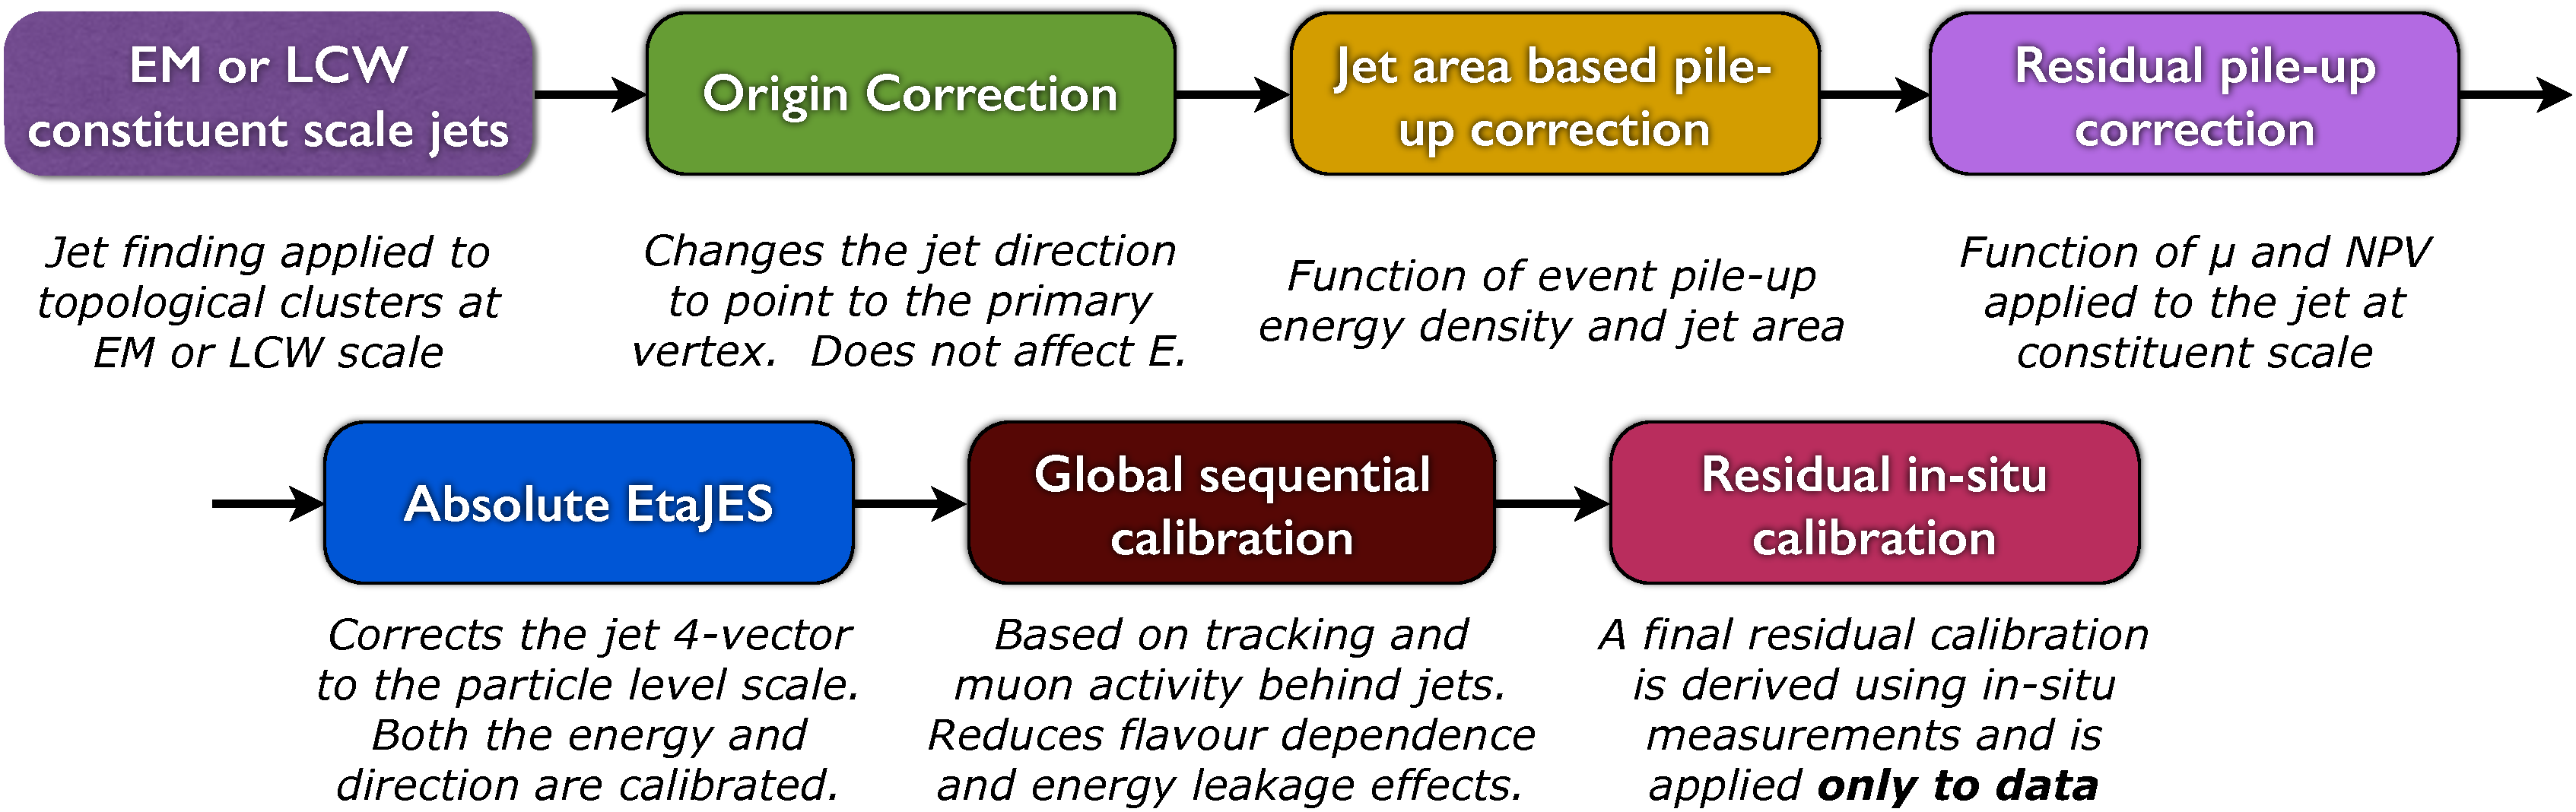
\includegraphics[width=0.85\textwidth]{figures/JetCalib/JetCalibFlow.png}\hspace{0.05\textwidth}
\end{center}
\caption{Flow chart of the steps involved in jet calibration. (Figure taken from \cite{Calibartion13TeV}) }
\label{fig:jetCalibFlow} 
\end{figure}

\indent First the individual topo-clusters in the jet are calibrated to the energy scale of EM showers using MC simulations.\cite{topoCalib}  It should be noted that this calibration is to EM showers correctly calibrates the energy in EM showers but underestimates the amount of energy lost in hadronic showers.  Additional corrections are applied in the following steps to account for this difference. \\
% The origin of the reconstructed jet is also set to the primary vertex instead of the default detector center. \\

\indent A correction for energy deposited by pileup interactions are applied.\cite{pileupsub}  The correction is based on the measurement of average energy originating from pileup $\rho$ multiplied by the measured jet area.  The pileup energy density is defined in equation \ref{eqn:PileupDensity} and determined by measuring the median energy density of $R=0.4$ $k_t$ jets found in the central $|\eta|<2.0$ part of the calorimeter.  The $k_t$ algorithm preferentially cluster soft objects first instead of hard objects and is more sensitive to soft pileup radiation and no $\pt$ thresholds are applied to the reconstructed $k_t$ jets as we are trying to measure soft objects.  \\

\begin{equation}
\rho=median\{ \frac{p_{T i}^{k_t~jet}}{A_i^{k_t~jet}} \}
\label{eqn:PileupDensity}
\end{equation}

\indent The area based pileup energy correction is subtracted along with two other residual corrections.  The total pileup correction to jet $\pt$ is given in equation \ref{pilupCorrection}. \\

\begin{equation}
p_T^{corr} = p_T - \rho \times A - \alpha~\times (N_{PV} - 1 ) - \beta~\times <\mu>
\label{eqn:pilupCorrection}
\end{equation}

\indent  It should be noted that the jet energy response still has a dependence on pileup after this area based correction has been applied.  The sources of this dependence can be attributed to the incomplete cancelation of in-time and out-of-time pileup.\cite{JetCalibartion13TeV}  For example, events with a low number of reconstructed vertexes ($N_{PV}$) in a run with high average number of interactions per bunch crossing ($<\mu>$) may receive relatively large amounts of out-of-time pileup compared to in-time pileup.  This effect is also parameterized by using the constants $\alpha$ and $\beta$ in equation \ref{pilupCorrection}. \\  

\indent In the next step, the jet energy scale (JES) is applied.  JES is a scale factor which relates the reconstructed jet energy with the true jet energy.  JES is calibrated using a number of MC and data driven methods.  The JES is derived from an inclusive jet MC after pileup and origin corrections have been applied.  \\

\indent A residual difference between the energy responses of gluon and light quark jets remains after JES calibration.\cite{JetCalibartion13TeV}  The difference can be as large as 8 percent and is due to a number of reasons including the factor of 2 difference in color charge between quarks and gluons.  A global sequential correction scheme (GSC) is applied to account for this deference and correct for other detector based issues.\cite{jet_GSC}  \\

\indent GSC corrections uses information on the topology of energy deposits, associated inner detector tracks and activity in the muon spectrometer behind the jet.  ID Tracking information is used to reduce the flavour dependence because gluon initiated jets tend to have a wider profile and more tracks. Muon spectrometer information is used to better estimate high energy jets which penetrate the full depth of the calorimeter.  Information on the relative amount of calorimeter energy deposited in specific layers is used to improve the jet energy resolution. \\

\indent Lastly, further corrections to the jet energy response are obtained by measuring the balance between jets and some reference objects directly in data. \cite{JES_ZGamma,JES_dijet}  The reference object can be a photon, a $Z$ boson or other jets.  The $\pt$ balance between jets and the reference objects are measured in data and compared to the MC.  A residual correction is applied by the data over MC ratio based on equation \ref{jet_insitu}.  Systematic uncertainties on the jet energy responses including those on the jet energy scale and jet energy resolution are also derived using these data driven methods. \\

\begin{equation}
\frac{R_{data}}{R_{MC}} = \frac{<p_T^{jet}/p_T^{ref}>_{data}}{<p_T^{jet}/p_T^{ref}>_{MC}}
\label{eqn:jet_insitu}
\end{equation}

\indent The jet $\pt$ resolution for $|\eta|<0.8$ and $0.8<|\eta|<1.2$ jets are shown in figure \ref{fig:jet_ptresolution}.\cite{JES_dijet} \\

\begin{figure}[htb]
  \begin{center}
    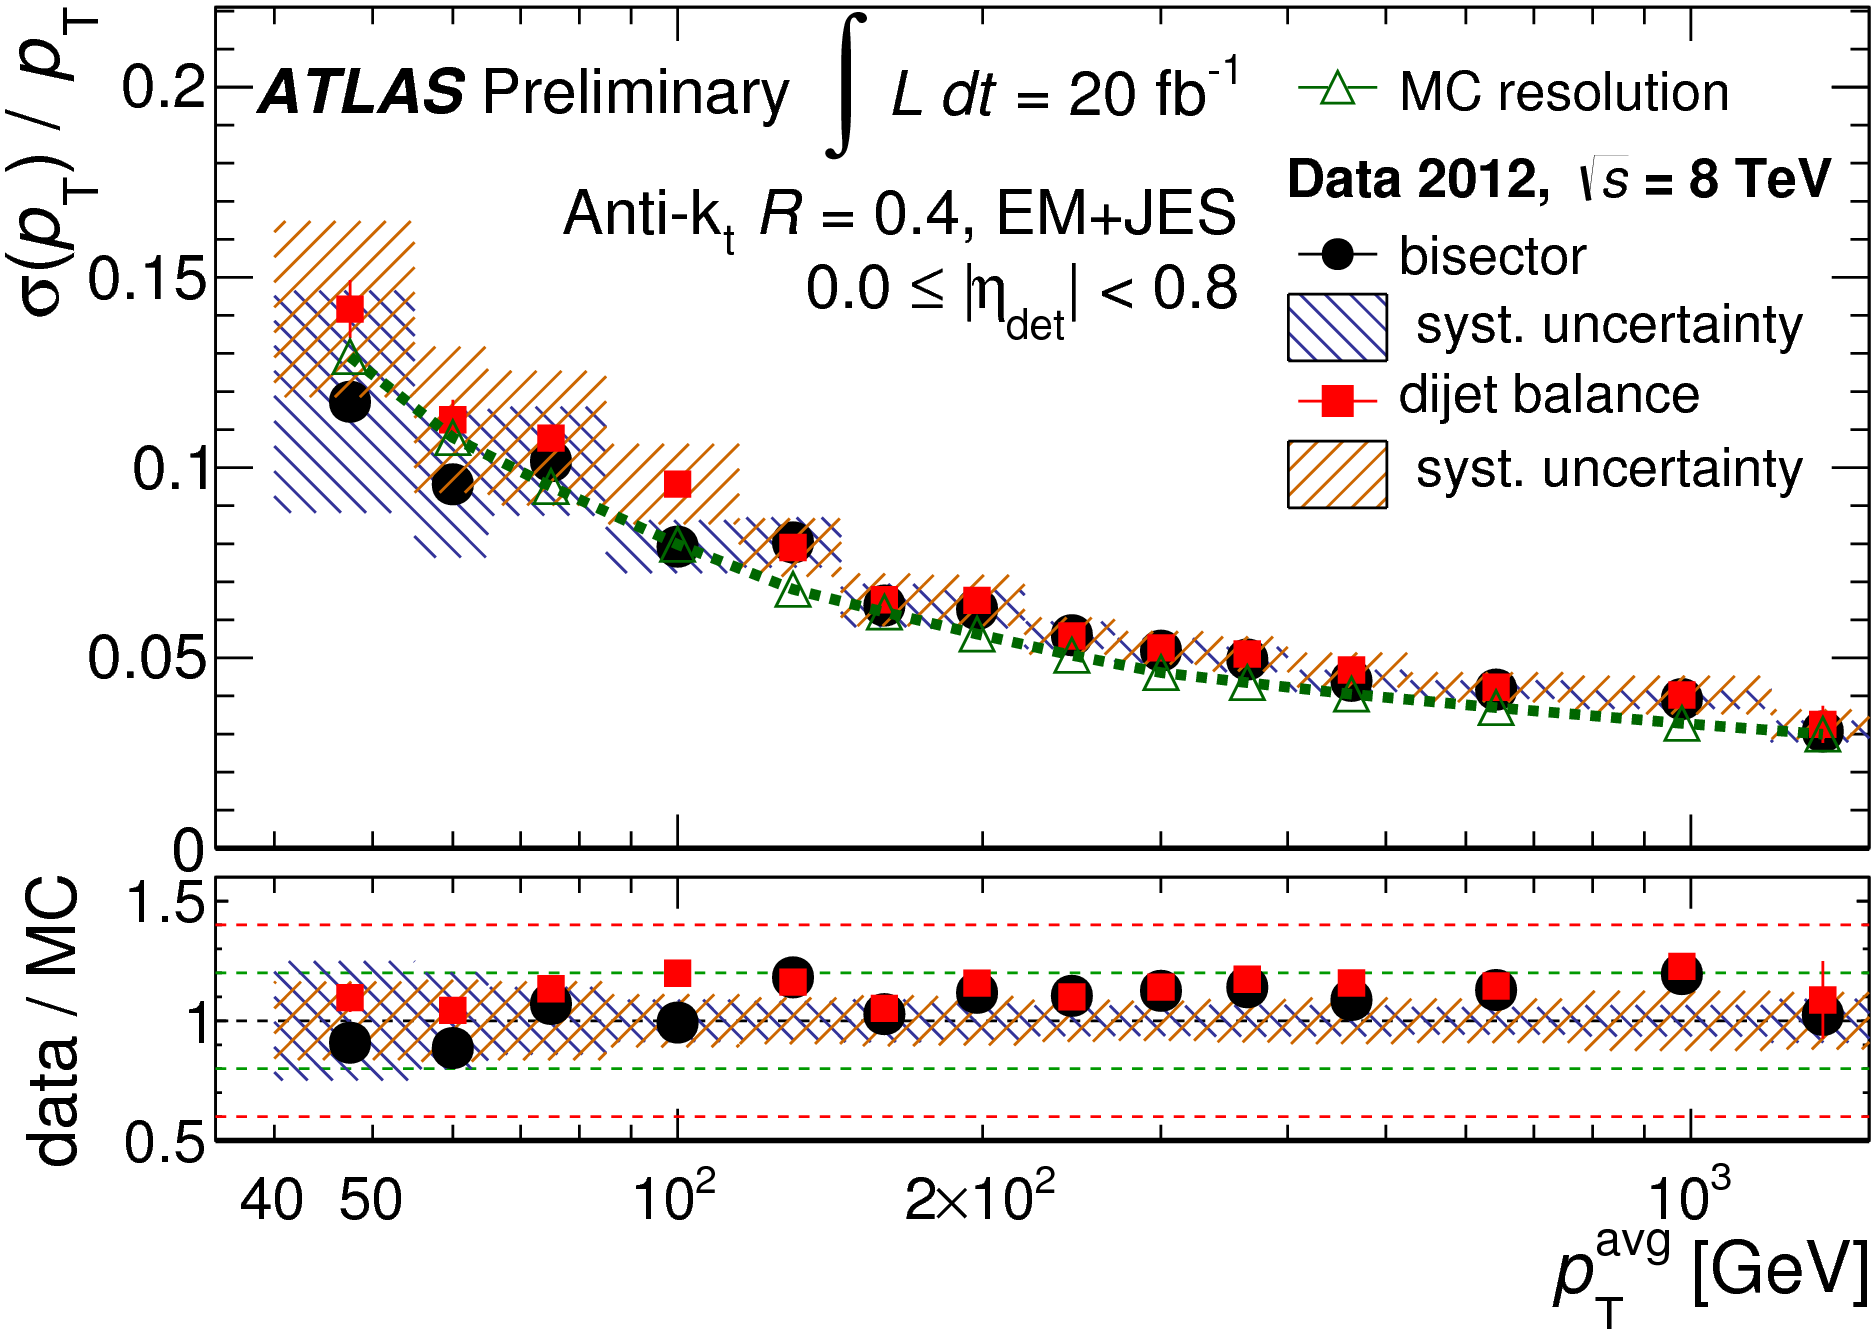
\includegraphics[width=0.45\textwidth]{figures/JetCalib/JetCentral_Response.png}\hspace{0.05\textwidth}
    \includegraphics[width=0.45\textwidth]{figures/JetCalib/JetTransition_Response.png}\hspace{0.05\textwidth}
\end{center}
\caption{Jet $\pt$ resolution for $|\eta|<0.8$ and $0.8<|\eta|<1.2$ jets as a function of jet $\pt$ in 8 TeV data. (Figure taken from \cite{JES_dijet}) }
\label{fig:jet_ptresolution} 
\end{figure}

\subsection{Pileup Jet Rejection and Jet Vertex Tagger}
\label{sec:jet:JVT}

\indent It is imperative to be able to distinguish between jets originating from the hard scattering interaction (hard scattering jets) and those originating from other pile-up interactions (pileup jets) in the high luminosity LHC environment.  Pileup jets may originate from both the on average 25 additional p-p interactions in the same bunch crossing or from interactions in other beam crossings.  We distinguish between the hard scattering jets from pileup jets using a multivariate discriminate known as the jet vertex tagger (JVT).\cite{JVT} \\

\indent The JVT discriminate is based on two variables $\corrJVF$ and $\RpT$ defined in equations \ref{eqn:corrJVF} and \ref{eqn:RpT}.

\begin{equation}
\corrJVF = \frac{\sum_i p_T^{trk_i} (PV_0) }{ \sum_l p_T^{trk_l} (PV_0) + \frac{\sum_{n\ge1} \sum_l p_T^{trk_l} (PV_n) }{k\dot n^{PU}_{trk}} }
\label{eqn:JVF}
\end{equation}

\begin{equation}
\RpT = \frac{\sum_i p_T^{trk_i} (PV_0) }{ p_T^{jet} }
\label{eqn:RpT}
\end{equation}

\indent The $\corrJVF$ variable roughly corresponds to the fraction of a jet's ID track $\pt$ that originate from the hard scattering vertex.  $\sum_i p_T^{trk_i} (PV_0)$ is the sum of all jet's associated track $\pt$ that originate from the primary vertex $PV_0$.  The quantity $p^{PU}_T = \sum_{n\ge1} \sum_l p_T^{trk_l} (PV_n)$ is the total amount of a jet's associated track $\pt$ that originates from pile up interactions.  $p^{PU}_T$ is divided by $k\dot n^{PU}_{trk}$ to correct for the fact that $<k\dot n^{PU}_{trk}>$ will increase linearly with the number of pileup vertexes $n^{PU}_{trk}$.  This makes the variable $\corrJVF$ roughly independent to the number of reconstructed vertexes. The value $k$ is set to an arbitrary $0.01$ and the discriminating power of JVT was found to be independent of the choice of $k$.\\

\indent $\RpT$ is defined as the total track $\pt$ of all associated tracks that originate from the primary vertex $PV_0$ divided by the fully calibrated jet $\pt$. It is important to note that the calibrated jet $\pT$ includes pileup subtraction.  $\RpT$ peaks sharply at zero for pileup jets.  On the other hand, $\RpT$ corresponds to roughly the charged $\pt$ fraction in hard scattering jets.  \\

\indent The JVT discriminate constructs a 2D likelihood based on these variables.   The JVT discriminate determines the probability that a jet will be a hard scattering jet using the k-nearest neighbor (kNN) multivariate technique \cite{TMVA} trained on a $20<\pt<50 \gev$ and $|\eta|<2.4$ MC sample of hard scattering and pileup jets.  The k-nearest neighbor (kNN) algorithm is robust relative to local fluctuations in sparsely populated regions.  \\

\indent For our analysis we require a jet vertex tagger value greater than 0.59.  This corresponds to a 92 percent efficiency for jets originating from the hard scattering interaction and a 2 percent fake rate from pileup jets, if the jet has $|\eta| < 2.4$ and $\pt < 60 \gev$.  The JVT efficiency as a function of jet $\pt$ is shown in figure \ref{fig:JVT_eff} \\

\begin{figure}[htb]
  \begin{center}
    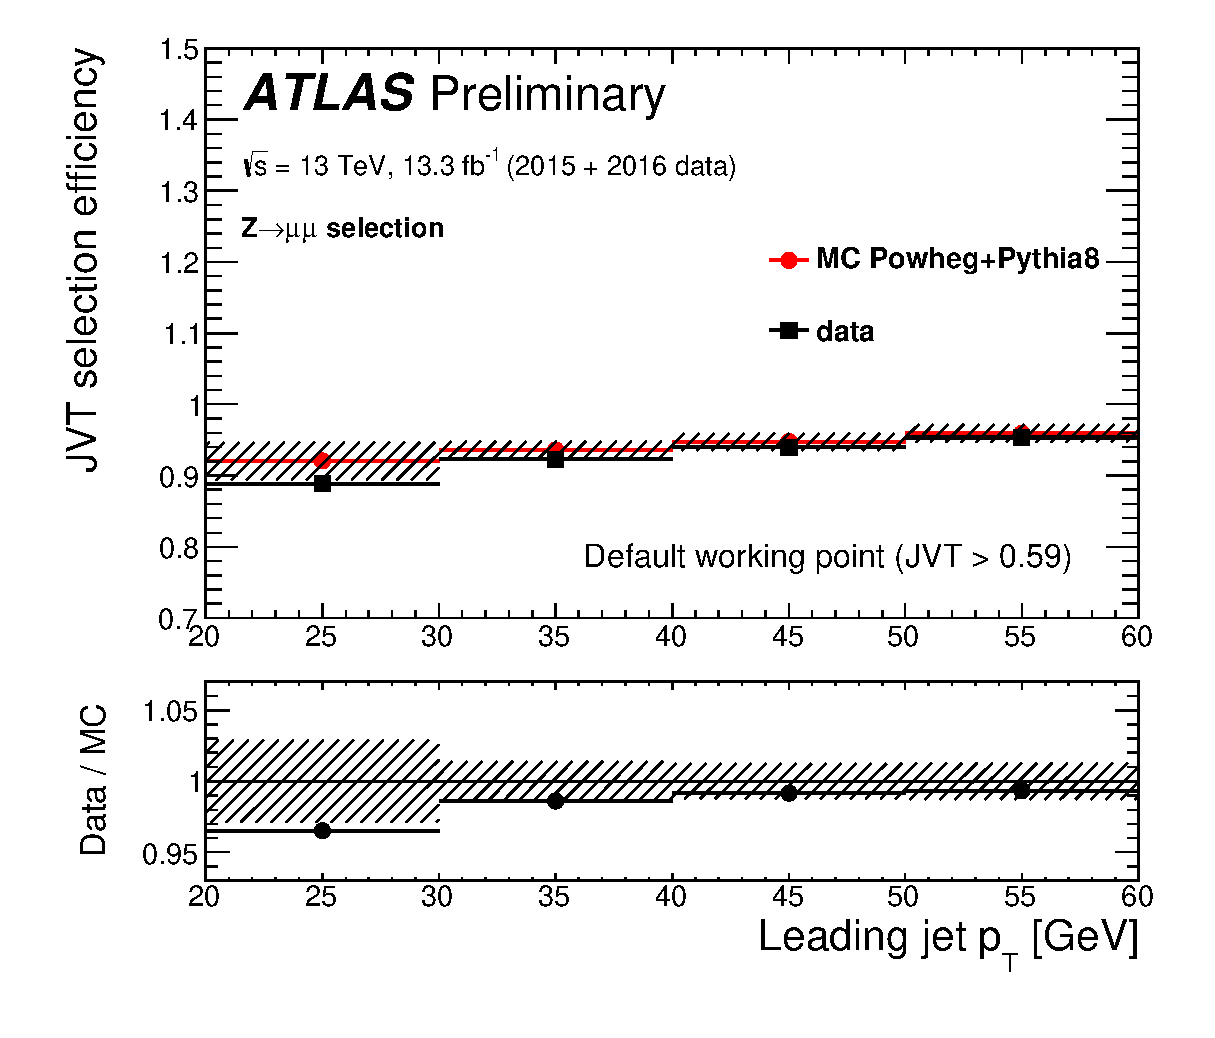
\includegraphics[width=0.65\textwidth]{figures/JetCalib/JVT_eff.eps}\hspace{0.05\textwidth}
\end{center}
\caption{The distribution showing the jet vertex tagger efficiency as a function of jet $\pt$ in 2015+2016 data. Only jets balanced against a $Z->\mu\mu$ boson are accepted.  Details can be found in \cite{JVT}. }
\label{fig:JVT_eff} 
\end{figure}

\subsection{Jet Quality and Jet Cleaning}
\label{sec:jet:quality}

\indent Several variables are useful in discriminating between real hadronic jets and fake jets not coming from p-p interactions.  The sources of fake jets include noise in the LAr and Tile calorimeters, beam induced backgrounds and cosmic raw showers.  These variables can be divided into three broad categories: variables quantifying the EM and hadronic calorimeter energy ratio, ID track based variables and variables based on the pulse shape of the LAr calorimeters.  Detailed descriptions of the variables used can be found in \cite{JetCleaning} a brief summary will be given here.\\

\indent Energy ratio variables can reject calorimeter noise and beam induced backgrounds and energy deposited from cosmic rays.  Jets originating from beam induced backgrounds tend to concentrate more energy in a few longitudinal layers compared to jets from p-p collisions.  Multiple variables corresponding to the fraction of jets energy deposition in any one section along the expected direction of the shower relative to the total energy deposition are useful in discriminating against fake jets. \\

\indent Energy ratio variables include: \\

\begin{itemize}
\item[] $f_{EM}$: ratio of EM calorimeter energy to total jet energy
\item[] $f_{HEC}$: ratio of HEC calorimeter energy to total jet energy
\item[] $f_{max}$: maximum energy fraction in any single calorimeter layer
\end{itemize}

\indent ID track based variables are useful because tracks can be matched to the primary vertexes in good jets.  Fake jets have low fraction of tracks which can be matched to primary vertexes.  \\

\indent list of track based variables include: \\

\begin{itemize}
\item[] $f_{ch}$: ratio of the scalar sum of ID track $\pt$ where ID track must originate from the primary vertex to jet $\pt$.  approximately the fraction of jet energy carried by charged particles.  
\item[] $f_{ch}/f_{max}$: ratio of $f_{ch}$ and $f_{max}$, the maximum energy fraction in any single calorimeter layer
\end{itemize}

\indent Pulse shape in the LAr should be consistent with those of a particle shower in good jets.  A quality variable $Q^{LAr}_{cell}$ measures the quadratic difference between expected and actual pulse shapes in each LAr cell.  Quality variables based on the fraction of cells in a jet with poor quality and the average quality is found to provide discrimination power against LAr noise. \\

\indent LAr pulse shape variables include: \\

\begin{itemize}
\item[] $\braket{Q}$: weighted average of pulse quality of LAr cells ($Q^{LAr}_{cell}$) in a jet.  Normalized to $0 < \braket{Q} < 1$.
\item[] $f^{LAr}_{Q}$: Fraction of energy in cells with poor quality pulse shapes in EM LAr Calorimeter
\item[] $f^{HEC}_{Q}$: Fraction of energy in cells with poor quality pulse shapes in hadronic endcap calorimeters (HEC) which also use LAr technology.
\item[] $E_{neg}$: total energy of all cells with negative energy
\end{itemize}

\indent A jet satisfying any one of the following criteria is considered a {\tt BadLoose} jet.  The presence of a {\tt BadLoose} can result in poor $\met$ reconstruction due to a noisy calorimeter or beam induced background.  Therefore, if any jet in the event is found to be {\tt BadLoose} then the entire event is rejected.   This procedure is called jet cleaning.  \\

\indent A jet is considered a {\tt Loose} jet if is not identified as a {\tt BadLoose} jet.  {\tt Loose} jets are used as signal jets in most ATLAS physics analysis including this one. \\

\begin{enumerate}
\item[] $f_{EM} > 0.5$ and $|f^{HEC}_{Q}| > 0.5$ and $\braket{Q} > 0.8$
\item[] $E_{neg} > 60 \gev$
\item[] $f_{EM} > 0.95$ and $f^{LAr}_{Q} > 0.8$ and $\braket{Q}>0.8$ and $|\eta|<2.8$
\item[] $f_{max}>0.99$ and $|\eta|<2.0$
\item[] $f_{EM}<0.05$ and $f_{ch}<0.05$ and $|\eta|<2$
\item[] $f_{EM}<0.05$ and $|\eta|\ge2$
\end{enumerate}

\subsection{Identifying Jets Originating from Heavy Flavor Hadrons}
\label{sec:jet:btagging}

\indent Hadrons containing b-quarks have long lifetimes, around 1.5 ps or a $c\tau$ of roughly 450 $\mu$m.  The long flight distance allows us to reconstruct ID tracks with large impact parameters and perhaps reconstruct secondary vertexes. \\% The typical b-hadron decay consist of at least one vertex displaced from the point of initial hard scattering.  \\

\indent Three separate algorithms have been setup to distinguish jets originating from b-hadrons (b-jets) from light hadrons and c-hadrons (c-jets).  A brief description of each algorithm is given in this section.  More details can be found in \cite{btagging2016}  and \cite{btagging2015}.  \\

\indent The first algorithm is based on track impact parameters for high quality tracks that are associated with jets.  The discriminate is computed as a sum of the log likelihood ratio of each accepted track in the vertex or $\sum_i \ln(\frac{p_b}{p_{light}})$, where i sums over all accepted tracks in the jet and $p_b$ is the PDF for a b-jet and $p_{light}$ is the PDF for a light jet.  The PDF uses transverse and longitudinal impact parameters $d_0$ and $z_0$ as observables and is derived from MC simulation.  \\

\indent The second algorithm seeks to reconstruct the secondary vertex associated with the b-hadron decay.  This algorithm has the advantage that if a secondary vertex is consistent with the decays of long lived hadrons that do not contain b-jets such as $K_s$ or $\Lambda$ or photon conversions then the vertex maybe rejected.  For example, secondary vertexes with a mass greater then $6 \gev$ are inconsistent with b decays and are rejected. Variables based on the secondary vertex location, energy, and mass can all be used to discriminate b-jets from light-jets and c-jets.  \\

\indent The third algorithm attempt to reconstruct the full b-hadron decay chain and is called the decay chain multi-vertex reconstruction algorithm.  The algorithm uses a Kalman filter to determine the common line on which the primary vertex and the bottom/charm vertexes lie.  \\

\indent The output of the three algorithms are all combined into a multivariate discriminate called MV2.  MV2 uses a boosted decision tree (BDT) algorithm \cite{TMVA} to gain better separation power between different jet flavors. This analysis uses the MV20c10 discriminate to tag b-jets. MV20c10 is selected as it gives the best balance between light jets and c-jet rejection for a given b-tagging efficiency.  \\

\indent The b-tagging efficiencies and mis-tag rates have been calibrated by the ATLAS flavor tagging group.  The distribution of the MV20c10 discriminate for light, charm and b-hadrons can be seen in figure \ref{fig:MV20c10}. We make a selection at MV2c10 $ > 0.6459$ which corresponds to approximately 77\% b-tagging efficiency with a factor of 134 reject rate for light jets.  \\

\begin{figure}[htb]
  \begin{center}
    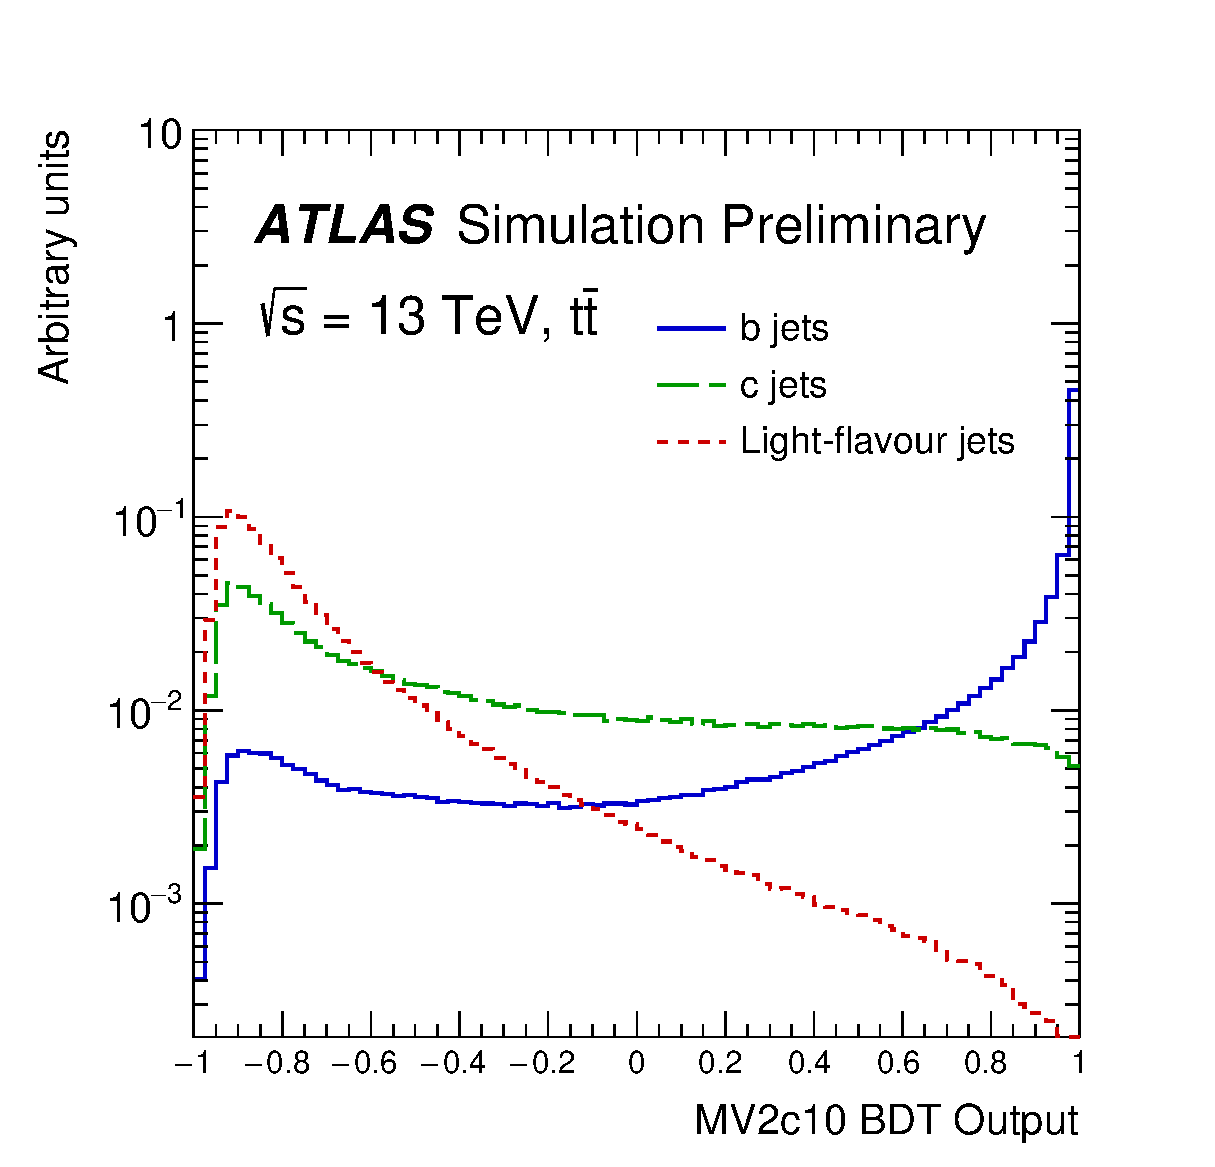
\includegraphics[width=0.85\textwidth]{figures/JetCalib/MV20c10.eps}\hspace{0.05\textwidth}
\end{center}
\caption{Distribution of the MV20c10 multivariate discriminate used for tagging b-jets.  Figure taken from \cite{btagging2016}  }
\label{fig:MV20c10} 
\end{figure}
